\subsection{Community Detection}
An important aspect of social network analysis is the detection of communities within a graph.

\subsubsection{Clustering}
Within social networks, there are distinct regions of vertices with many connections passing between them, and a much smaller number connected to other vertices outside of this region. These regions are termed as \emph{clusters}.

Social networks are a prime example of this. A person tends to have groups of friends distinct from each other, and friends within these groups are also friends of each other. Figure \ref{fig:socialnetwork} is a social network constructed from data regarding mutual friends of a person. Within this Figure, it can clearly be seen that there exists five distinct regions of mutual friends, with very few links between these regions. These regions are the clusters described above.

With data presented in this manner, it is clear to an observer where these clusters exist, and how many distinct clusters there are. \cite{girvan02} presents an approach to identifying communities within a graph.

\begin{figure}[htbp]
\centering
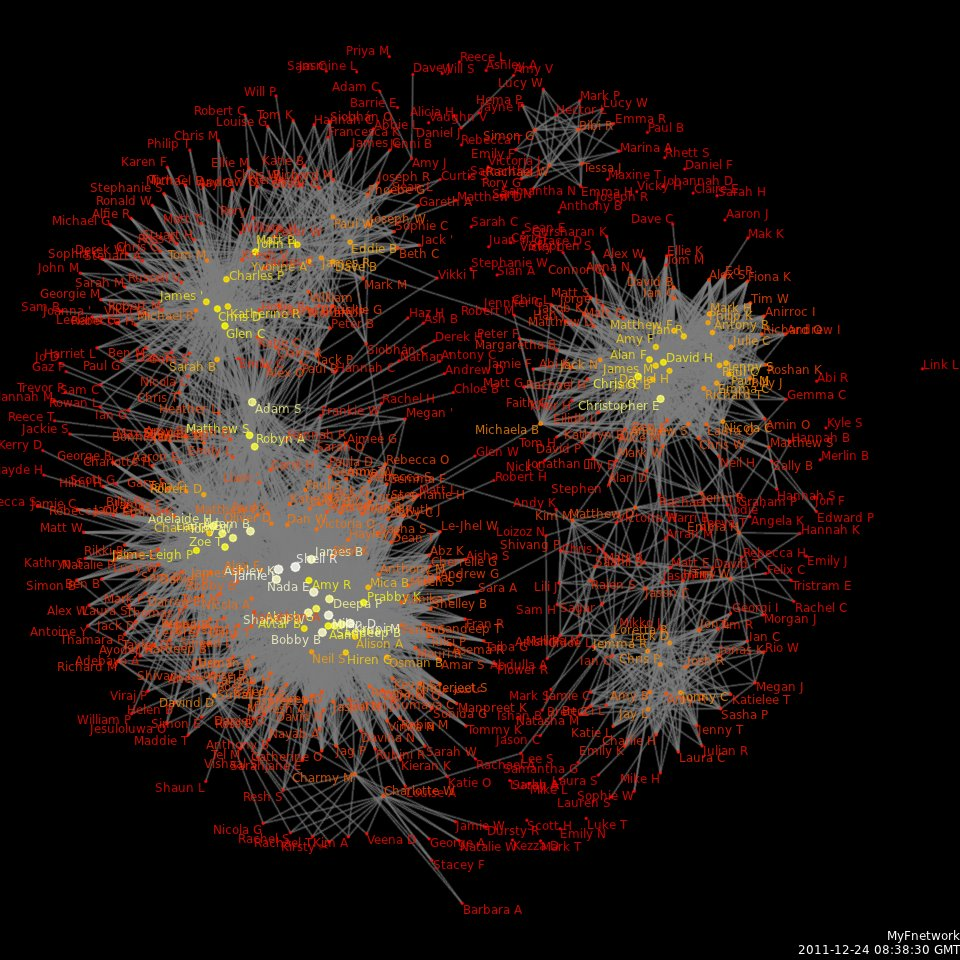
\includegraphics[width=0.5\textwidth]{./img/socialnetwork.png}
\caption{Social Network constructed from Facebook friends using the myFnetwork app}
\label{fig:socialnetwork}
\end{figure}

\subsubsection{\emph{k}-Cliques}
The term $clique$ is introduced by \citeauthor{luce49} in \cite{luce49} to describe a subgraph which consists of at least three vertices, each of which are fully connected with each other. From a social network perspective, this translates to saying that for each person in the clique, all of their friends  within the clique are friends of each other as well.

A \emph{k}-clique is defined as a clique which has size \emph{k}. A \emph{maximal clique} is a clique to which no more vertices can be added without violating the conditions of a clique, and the maximum clique is a clique within a graph which contains the largest number of vertices.

\begin{figure}[htbp]
\centering
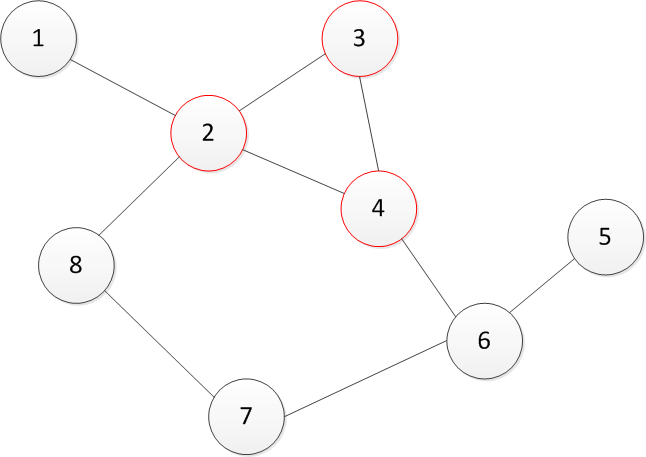
\includegraphics[width=0.5\textwidth]{./img/clique.png}
\caption{Graph highlighting a 3-clique}
\label{fig:clique}
\end{figure}

Figure \ref{fig:clique} shows an example graph highlighting a 3-clique. It has one maximum clique \{2,3,4\} which is highlighted in red, and six other maximal cliques \{1,2\}, \{2,8\}, \{4,6\}, \{5,6\}, \{6,7\}, \{7,8\}.

\begin{figure}
  \centering
  \subfloat[3-clique]{\label{fig:gull}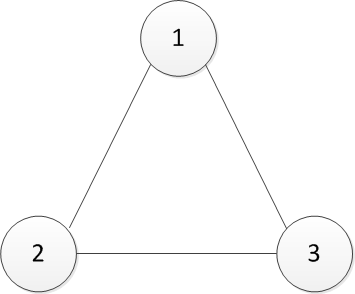
\includegraphics[width=0.3\textwidth]{./img/3-clique}} ~ \subfloat[4-clique]{\label{fig:tiger}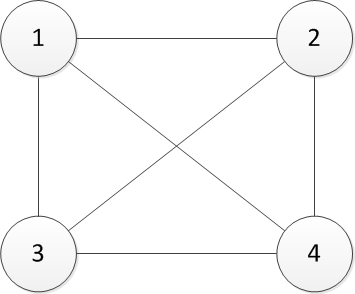
\includegraphics[width=0.3\textwidth]{./img/4-clique}} ~ \subfloat[5-clique]{\label{fig:mouse}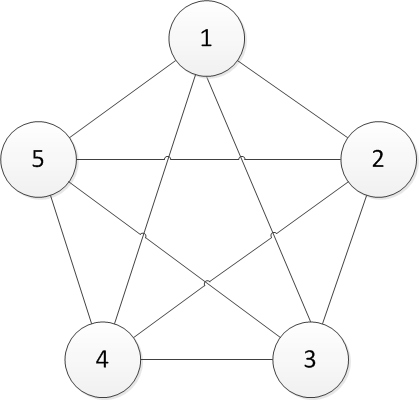
\includegraphics[width=0.3\textwidth]{./img/5-clique}}
  \caption{\emph{k}-cliques}
  \label{fig:cliques}
\end{figure}

Identifying cliques, and solving problems involving cliques as been shown to be computationally hard \cite{bomze99, trusses}. Cliques are either too common, with cliques of only a few members are frequently too numerous to be helpful, or too rare, with large cliques too limiting to be of use \cite{trusses}. Also, computation of identifying cliques scales worse than any polynomial of the problem size, making the process unfeasible for large graphs \cite{trusses, bron72}.

There have been numerous generalisations of the clique construct to improve usefulness of the clique through relaxation of some of the properties of the clique. These include the \emph{n}-clique \cite{luce50}, \emph{n}-clan \cite{alba73} and \emph{n}-club \cite{mokken79}. However these new constructs do not solve the issues of identifying cliques, and remain hard to compute and produce too many results.

\subsubsection{\emph{k}-Trusses}
Following from relaxing properties of the clique, \citeauthor{trusses} in \cite{trusses} introduces a new construct called a truss. A \emph{k}-truss is a subgraph where an edge between two vertices, A and B, exists if at least \emph{k-2} other vertices are connected to both of A and B. The \emph{k}-truss has similar definitions to the clique. A maximal \emph{k}-truss is a \emph{k}-truss that is not a proper subgraph of another \emph{k}-truss.

\begin{figure}[htbp]
\centering
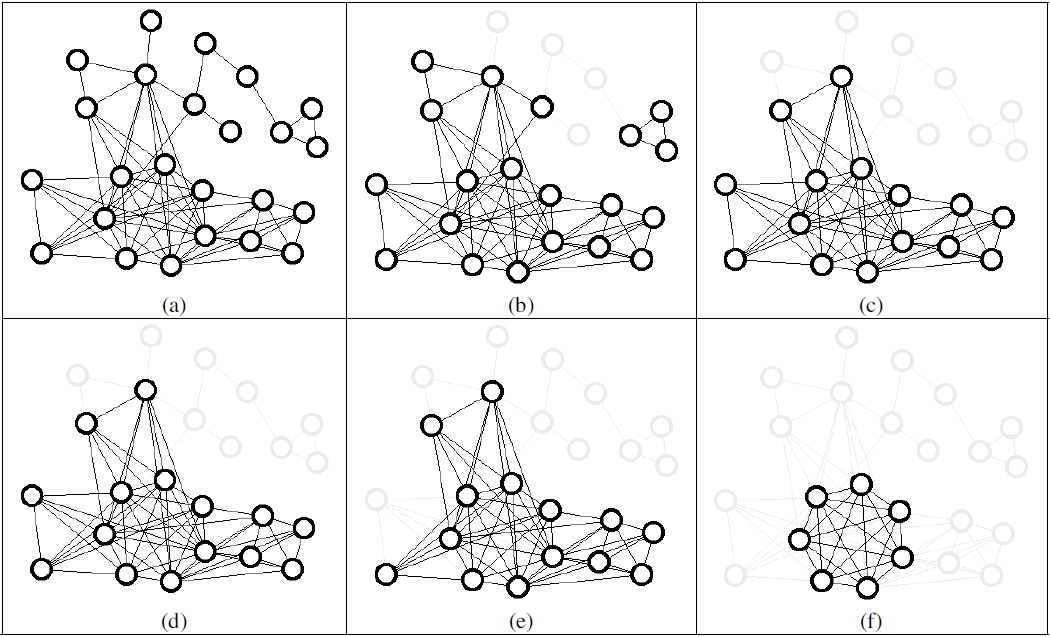
\includegraphics[width=0.9\textwidth]{./img/trusses.png}
\caption{An Example of Maximal Trusses. (a) original graph, (b) 3-trusses, (c) 4-truss, (d) 5-truss, (e) 6-truss. Note that (c) and (d) are the same. \cite{trusses}}
\label{fig:trusses}
\end{figure}

Figure \ref{fig:trusses} shows an example application of \emph{k}-trusses. Figure \ref{fig:trusses}(a) shows the original graph. Figures \ref{fig:trusses}(b-f) show the \emph{k}-truss for increasing values of \emph{k}. If the same original graph were to be analysed for \emph{k}-cliques for the same values of \emph{k}, more vertices in the graph would have been removed in earlier stages, which would have lost the interesting stage where Figures \ref{fig:trusses}(c) and (d) are identical.

The \emph{k}-truss is also computable in polynomial time to the input graph, which offers a marked improvement on the computation costs of identifying cliques and similar constructs. \cite{trusses} shows that the naive algorithm  for computing maximal \emph{k}-trusses is bounded by $O(n|E|^2 + n)$, where \emph{n} is the number of vertices in the graph, and \emph{|E|} is the number of edges in the graph. A more efficient method is shown to take $O(\Sigma d^2(v))$, where \emph{d(v)} is the degree of a vertex, \emph{v}.

\subsubsection{Clustering Coefficients}
Clustering coefficients provide a way to measure the amount to which vertices within a graph cluster together.